\section{Dégagement des contraintes de développement}

Selon des fonctions définies et des codes existantes, j'ai défini des contraintes et proposé des solutions :


\subsection{La gestion d'utilisateurs}

\textbf{Contraintes} 

\begin{itemize}
    \item Manque d'un système d'accès connecté celui de l’écoles
    \item Sans reconnaissance d’identités
\end{itemize}

J'ai proposé :

\begin{itemize}
    \item Communiquer avec les responsables informatiques d'écoles pour intérroger des méthodes de connection
    \item Réaliser la reconnaissance selon les mails address \footnote{ Par exemple, @eleves.ec-nantes.fr indique un élève et @ec-nantes.fr indque un enseignant } 
    \item Avant l'intégration de comptes, un système d'autorisation provisoire ressemblant celui d'ezb sera réalisé
    \item Des messageries à ajouter supplémentairement à la fin
\end{itemize}


\subsection{La gestion de livre}

\textbf{Contraintes} est :Manque de possibilités d'utilisation de multi-format et téléchargement.

J'ai proposé :

\begin{itemize}
    \item Sauvegarder des fichiers en format XML, TEI précisement, pour sa utilisation générale dans le domaine de livre numérique
    \item Chercher des outils de transformations, sinon il faut fabriquer un 
    \item Permettre le créateur d'un livre de définir son status, publique ou privé, pour éviter des problèmes de copyright
\end{itemize}


\subsection{La gestion de groupes}

\textbf{Contraintes} :Trop de niveaux à choisir quand ajouter un membre qui comprend même le niveau Créateur.

J'ai proposé :Ajouter des membres sans définir leur rôle, ne choisir qu'un seul membre comme le manager du groupe.


\subsection{La gestion de projets}

\textbf{Contraintes}

\begin{itemize}
    \item Impossibilité de définir la finalité par utilisateurs et de les distribuer aux sous-groupes
    \item Difficulté d'organiser des citations, résumés, écritures créatives, etc dans un layer
    \item Manque des contrôles de layers et des possibilité d'inviter des autres éditeurs hors du groupe
\end{itemize}

La nouvelle conception de l'application peut être présentée dans trois parties principales, la structure de projets, la distribution de projets et la contribution de projets.

\begin{figure}[H]
\centering
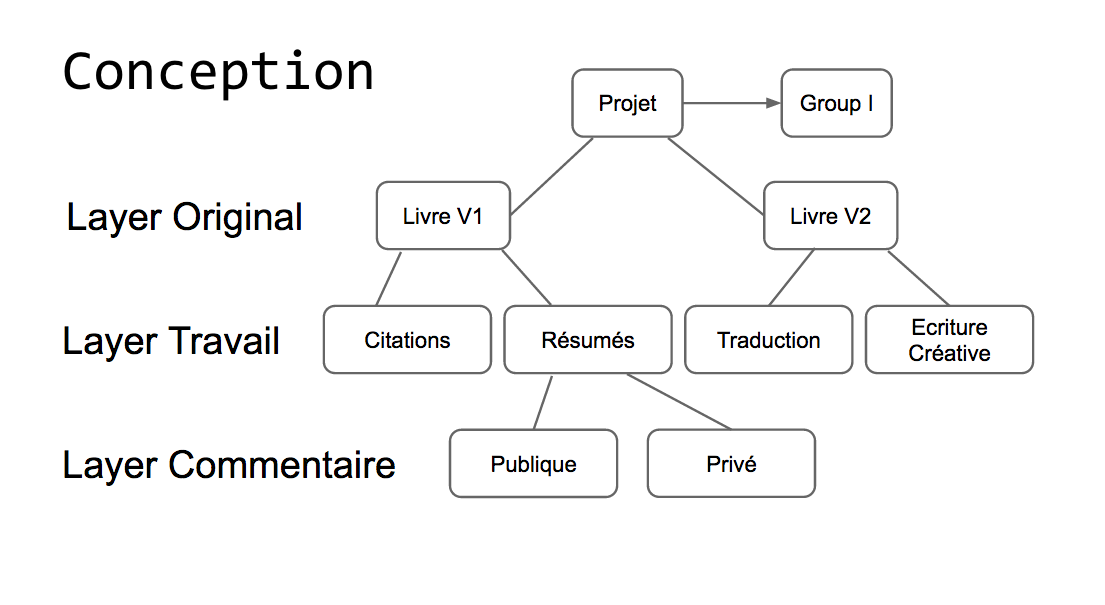
\includegraphics[width=\textwidth]{conception1}
\caption{Structure de projets}
\end{figure}

\begin{figure}[H]
\centering
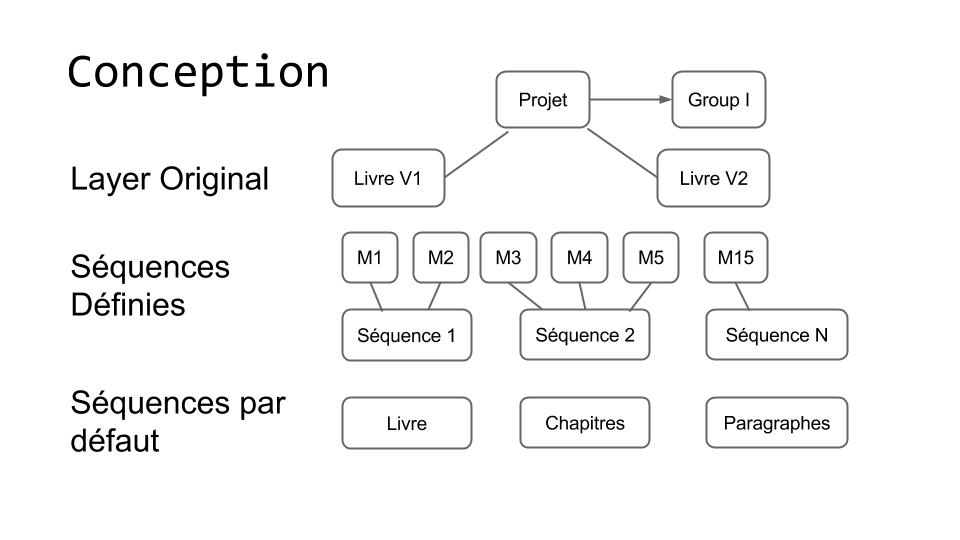
\includegraphics[width=\textwidth]{conception2}
\caption{Distribution de layers}
\end{figure}

\subsubsection{La structure de projets}

Pour garder la flexibilité de multi-échelles et la possibilité de création de layers contenant des citations et autres écritures, j'ai proposé un compromis :

\begin{itemize}
    \item Possible de choisir Privé comme le status d'un layer qui sera invisible pour le publique ni copi-able
    \item Livres sont traités comme layers originals où et on peut définir des marqueurs et des séquences dessus
    \item On peut créer autant de layers travails de manière multi-échelles 
\end{itemize}

\subsubsection{La distribution de projets}

Un autre problème des deux conceptions existantes est de ne pas pouvoir couper un livre dans plusieurs morceaux et les distributer aux sous-groupes d'élèves selon l'esprits d'enseignants. En même temps, il faut fournir des choix de finalités raisonnables automatiquement pour éviter trop de travail. Selon les contraintes, j'ai proposé :

\begin{itemize}
    \item Introduire les conception \textbf{Marqueur}, qui indique une position dans le livre, et \textbf{Séquence}, qui permet de choisir un marqueur au début, un à la fin et des élèves d'édition
    \item Permettre d'un distribution d'autres finalités fournies automatiquement par la plate-forme comprenant entier livre ou chapitres ou paragraphes, etc...
\end{itemize}

\subsubsection{La contribution de projets}

\begin{itemize}
    \item Quand créer un sous-layer d'un layer original, on peut sélecter une des toutes finalités possibles, des sous-layers d'un layer travail vont hériter sa finalité automatiquement
    \item Fournir plusieurs choix de type d'édition quand créer un layer :
            \begin{itemize}
                \item \textbf{Individuel} :une édition du créateur, des membres de groupe n'ont pas le droit d'éditer
                \item \textbf{Groupe} :une édition de groupe selon la distribution de la finalité du layer, un éditeur ne peut pas voir des éditions d'autres parties
                \item \textbf{Collaborative} :une édition synchronisée qui permet de lire des éditions d'autres parties mais ils ne peuvent éditer que dans la partie autorisée
            \end{itemize}
    \item Des éditions d'un layer travail sont des ajouts de parties qui permet des citations de parent-layer, des insertions et des écritures multiformat
    \item Dans des éditions d'un layer de niveau N, permettre de lire tous les layers de niveau original au niveau N-1
\end{itemize}

\begin{itemize}
    \item \textbf{Layers originals} représentant des livres sont des bases de projets
    \item \textbf{Layers travail} garantissent une structure multi-échelles illimité et des écritures très libres
    \item D'ailleurs, la nouvelle conception de projets permet d'inviter des autres personnes pour contribuer dans le projet ou commenter des travails faits par des élèves. 
\end{itemize}